\chapter{Vertices and Transforms}%{Philip Rideout}
\label{ch2}

\begin{figure}[htb]\centering
  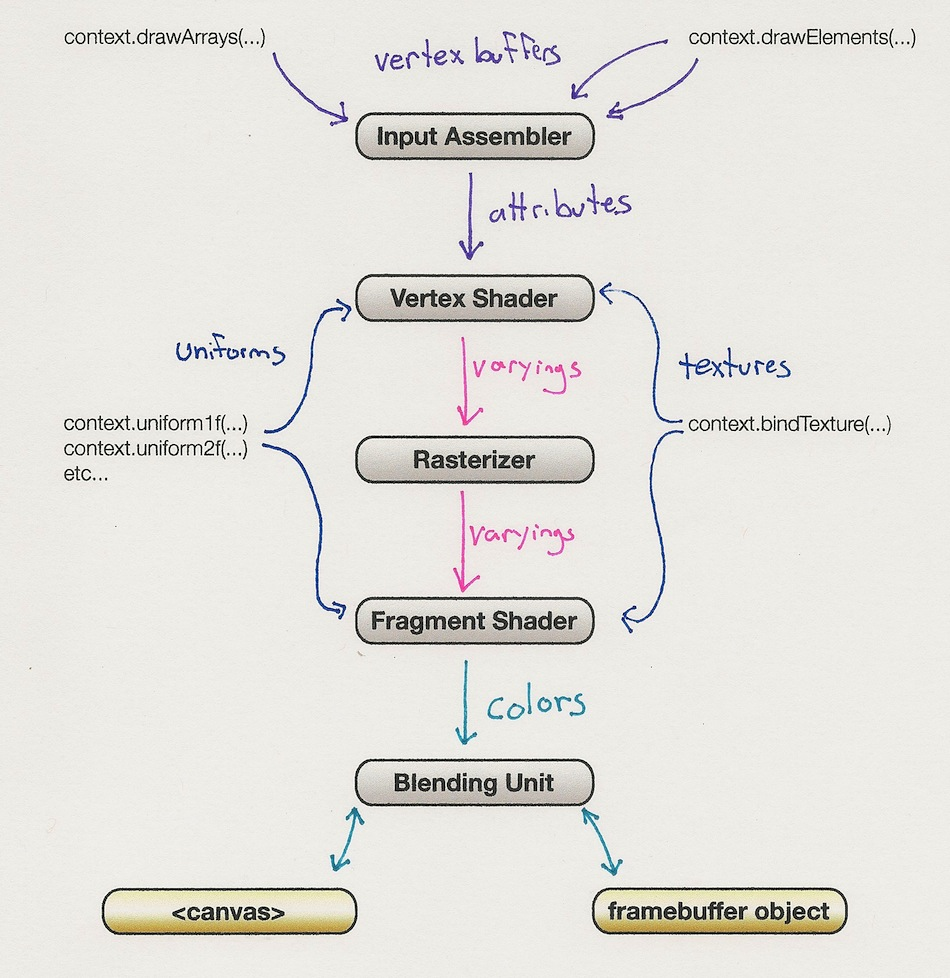
\includegraphics[width=70mm]{pipeline.jpg}
  \caption{High level view of the WebGL / OpenGL ES pipeline}
  \label{fig:AssemblyLine}
\end{figure}

%%%%%%%%%%%%%%%%%%%%%%%%%%%%%%
\section{WebGL at 10,000 feet}
\summary{High-level overview of the WebGL rendering pipeline.}

Earlier we mentioned that only two WebGL functions that can actually render 3D geometry: \code{drawArrays} and \code{drawElements}.  Both of these simply push a set of \index{vertices} vertices into the WebGL pipeline.  The vertices become rasterized into \index{fragments} \term{fragments}, or pixel values in the canvas.  Every vertex is defined by a set of \term{vertex attributes}, one of which is usually an XYZ coordinate.  Vertices come together to form \term{primitives}, which include point sprites, lines, and triangles.

Vertices initially belong to a swath of memory called a \term{vertex buffer}, and WebGL provides a rich API that allows you to specify how heterogenous attributes can be packed into a vertex buffer.  Figure~\ref{fig:AssemblyLine} depicts how vertex data flows through the pipeline, starting off in vertex buffers, eventually transforming into pixels in the canvas.

Two phases of this data flow are programmable: the vertex shader and the fragment shader.  Shaders are bundled together into \index{program object} \term{program objects}.   More precisely, a program object is the linked combination of a compiled vertex shader, a compiled fragment shader, a set of bindings for constant inputs (\term{uniforms}), and a set of bindings for vertex-varying inputs (\term{attributes}).

We'll dive deeper into shaders and vertex buffers later in this chapter; for now, see Listing~\ref{lst:Taste} for a taste of the various set-up that must be performed before actually pushing the vertices into the pipeline.

\begin{lstlisting}[
    caption={The typical state-setting that occurs before \code{drawArrays}.},
    escapechar=\%,
    label=lst:Taste,
    language=JavaScript]
// Bind a program object and set up a couple uniforms.
gl.useProgram(program);
gl.uniform1f(program, shininess, 0.5);
gl.uniform4fv(program, color, [1,1,0,1]);

// Bind a vertex buffer and set up the position attribute.
gl.bindBuffer(gl.ARRAY_BUFFER, buffer);
gl.enableVertexAttribArray(attribs.POSITION);
gl.vertexAttribPointer(attribs.POSITION, 3, gl.FLOAT, false, 0, 0);

// Finally, draw two triangles (six vertices), starting at vertex 0.
gl.drawArrays(gl.TRIANGLES, 0, 6);
\end{lstlisting}

%%%%%%%%%%%%%%%%%%%%%%%%%%%%%%%%%%%%%%%%
\section{Vector Algebra with JavaScript}
\notetoself{This sections walks through giza's implementation of vector and matrix classes.  Rotation, translation, and scale are given a very brief treatment.}

%%%%%%%%%%%%%%%%%%%%%%%%%%%%%%%%%%%%%
\section{The Typical Life of a Vertex}
\notetoself{Describes model, view, and projection transforms.}

%%%%%%%%%%%%%%%%%%%%%%%%%%%%%%%%%
\section{Shading Language Basics}
\notetoself{Explains uniforms, attributes, and varyings.  Walks through trivial \texttt{main} functions for vertex and fragment shaders.}

%%%%%%%%%%%%%%%%%%%%%%%%%
\section{Program Objects}

\subsection{Fetching and Compiling Shader Strings}

Shaders are specified with multi-line strings that get passed to WebGL for compilation.  There are several ways to embed a multi-line string in JavaScript code: you can end each line with a backslash, or concatenate a series of single-line strings with the \code{+} operator, or create an array of strings that become glued together with \code{join}.

None of embedded options are ideal, so another idea is to download the entire shader from an external file.  With jQuery, this is easily accomplished with \code{\$.get}.

In this book's sample code however, we've decided to use the HTML file as a container for all shader strings by authoring the shaders inside \code{<script>} elements.  Embedding arbitrary strings in \code{<script>} is also a common practice with templating systems such as \mbox{\code{handlebars.js}}.

Listing~\ref{lst:embed} shows how we embed a fragment shader in HTML.

\begin{lstlisting}[
    language=HTML,
    caption={Embedding a shader string in HTML.},
    label=lst:embed]
<script id="simplefs" type="x-shader/x-fragment">
  precision highp float;
  varying vec3 vColor;
  void main() {
      gl_FragColor = vec4(vColor, 1.0);
  }
</script>
\end{lstlisting}

With this system, every shader string is assigned a unique identifier in its enclosing script tag.  The string can then easily be retrieved using jQuery:

\begin{lstlisting}[language=JavaScript]
var fsText = $('#simplefs').text();
\end{lstlisting} % $

Alternatively, you can fetch the string through the raw DOM element:

\begin{lstlisting}[language=JavaScript]
var fsText = document.getElementById('simplefs').innerHTML;
\end{lstlisting}

After obtaining a shader string, the next step is to pass it into a WebGL shader object and compile it:

\begin{lstlisting}[language=JavaScript]
var fsObject = gl.createShader(gl.FRAGMENT_SHADER);
gl.shaderSource(shaderObject, fsText);
gl.compileShader(fsObject);
var status = gl.getShaderParameter(fsObject, gl.COMPILE_STATUS);
if (!status) {
 console.error(gl.getShaderInfoLog(fsObject));
}
\end{lstlisting}

Since GLSL does not have a \code{\#include} statement, it's often useful to stitch together several strings to form a single shader.  This allows you to share a single function (or block of uniforms) among several shader objects.  See Listing~\ref{lst:GIZA:compileShader} for Giza's implementation of a utility function that takes a list of ids and a shader type.  It fetches the strings from the DOM, glues them together, and compiles them.

\begin{lstlisting}[
    language=JavaScript,
    caption={The \code{compileShader} function (error checking omitted).},
    label=lst:GIZA:compileShader]
GIZA.compileShader = function(ids, type) {
  var gl = GIZA.context;
  var sourceText = "";
  for (var i = 0; i < ids.length; i++) {
    sourceText += document.getElementById(id).innerHTML;
  }
  var shaderObject = gl.createShader(type);
  gl.shaderSource(shaderObject, sourceText);
  gl.compileShader(shaderObject);
  return shaderObject;
};
\end{lstlisting}

\subsection{Creating Program Objects}

Recall that a \index{program object} program object is the linked combination of a compiled vertex shader, a compiled fragment shader, and a set of bindings for uniforms and attributes.

Giza provides a utility function that takes two id lists (one for the vertex shader, one for the fragment shader), aggregates them, compiles them, and links them into a program object.  See Listing~\ref{lst:GIZA:compileProgram} for the skeletal implementation -- we'll flesh it out a bit in upcoming sections.

\begin{lstlisting}[
    language=JavaScript,
    caption={The \code{compileProgram} function (abridged).},
    label=lst:GIZA:compileProgram]
GIZA.compileProgram = function(vsIds, fsIds) {
  var gl = GIZA.context;
  var vShader = GIZA.compileShader(vsIds, gl.VERTEX_SHADER);
  var fShader = GIZA.compileShader(fsIds, gl.FRAGMENT_SHADER);
  var program = gl.createProgram();
  gl.attachShader(program, vShader);
  gl.attachShader(program, fShader);
  // bind attributes here...
  gl.linkProgram(program);
  var status = gl.getProgramParameter(program, gl.LINK_STATUS);
  if (!status) {
    console.error("Could not link " + vsIds + " with " + fsIds);
  }
  // query uniforms here...
};
\end{lstlisting}

\subsection{Binding Vertex Attributes}

WebGL needs to know how to correllate data elements in the vertex buffer with attributes in the vertex shader.  Each attribute that the vertex shader reads has an associated string name and an associated integer handle.  The integer handle is used when specifying the vertex buffer layout, as you'll see in Section~\ref{sec:VBOs}.

WebGL and other OpenGL-based APIs provide two ways of associating attributes with integers: you can let WebGL make the association, or you can bind them explicitly.  To allow WebGL to make the association, just compile and link the program object as you normally would, then query for the integer handles afterwards like so:

\begin{lstlisting}
var handle = gl.getAttribLocation(programObject, "Position");
\end{lstlisting}

However, I generally try to avoid this strategy, preferring instead to bind attributes explicitly using WebGL's \code{bindAttribLocation} method:

\begin{lstlisting}
var handle = 3;
gl.bindAttribLocation(programObject, handle, "Position");
\end{lstlisting}

My usual approach is to specify a single, authoratative enumeration of all possible vertex attributes used in my application; this allows me to decouple vertex buffer layouts from shaders.  In other words, I can more easily mix and match vertex buffers with shaders.  This practice is known as \index{semantic binding} \term{semantic binding} in the OpenGL community.

For example, suppose your application creates two program objects: one that applies a texture, and another that performs lighting (both of which we'll learn about in future chapters).  The texturing program requires two attributes: positions and texture coordinates.  The lighting program requires positions and normal vectors.  With semantic binding, your application would define an object for the superset of these attributes:

\begin{lstlisting}
var attribs = {
  POSITION: 0,
  NORMAL: 1,
  TEXCOORD: 2
};
\end{lstlisting}

See Listing~\ref{lst:GIZA:compileProgram2} for how we augmented Giza's \code{compileProgram} method to read through a list of semantic attributes and explictly bind them.  Notice that we added a third argument to the function declaration.

\begin{lstlisting}[
    language=JavaScript,
    caption={Adding attribute binding to \code{compileProgram}.},
    label=lst:GIZA:compileProgram2]
GIZA.compileProgram = function(vsIds, fsIds, attribs) {
  ...
  for (name in attribs) {
    var handle = attribs[name];
    gl.bindAttribLocation(program, handle, name);
  }
  gl.linkProgram(program);
  ...
};
\end{lstlisting}

\begin{sidenote}%
Notice in Listing~\ref{lst:GIZA:compileProgram2} that the \code{bindAttribLocation} call occurs after shader compilation but before program linking.  WebGL requires attrributes to be bound before linking; this is a common gotcha!
\end{sidenote}%

\subsection{Querying and Setting Uniforms}

The other type of input data consumed by shaders are uniform variables.  Uniforms are constant across all vertices submitted to the draw call.  Similar to vertex attributes, uniforms have associated string names and locations.  However, uniform locations are opaque objects rather than integers.  The location of a uniform can be queried from the program object like so:

\begin{lstlisting}
var clipMatLoc = gl.getUniformLocation(programObject, "ClipMatrix");
\end{lstlisting}

The values for all uniforms are zero-filled by default, and can be set using any of the thirty \code{uniform*} methods available on the WebGL context.  Some examples of setting uniforms:

\begin{lstlisting}
gl.uniform1i(programObject, enableLightingLoc, 1);
gl.uniform2f(programObject, windowSizeLoc, 200.0, 100.0);
gl.uniform2fv(programObject, windowSizeLoc, [200, 100]);
gl.uniformMatrix3fv(programObject, clipMatLoc, false, clipMatValue);
\end{lstlisting}

There are a total of thirty functions for setting uniforms, but they all basically do the same thing.  The number (1-4) specifies the dimension of the vector; the \code{i} or \code{f} letter specifies the type (integer or float) and the the \code{v} suffix is used for passing a JavaScript sequence or typed array instead of separate arguments for each vector element.

Matrices are somehow special in that they are named \code{uniformMatrix*} and the specified dimension can only be 2, 3, and 4.  These functions also take an additional argument, which is boolean that can be set if you wish to transpose the matrix on the way down.

Wouldn't it be nice if you didn't have to query for location handles, and instead refer directly to the string name when setting a value?  We can make life easier by employing the age-old JavaScript trick of adding arbitrary properties to an API object.  For each uniform in the shader, we can graft a property onto the WebGL program object.  This will allow to set uniform values using a shorthand notation like this:

\begin{lstlisting}
gl.uniform1f(program, program.shininess, 3.0);
\end{lstlisting}

We usually stay away from mutating API objects in this way, but in this case we made an exception.  See Listing~\ref{lst:GIZA:compileProgram3} to see how \code{compileProgram} is enhanced to automatically graft all uniform locations onto the program object.

\begin{lstlisting}[
    language=JavaScript,
    caption={Grafting uniform locations onto the WebGL program object.},
    label=lst:GIZA:compileProgram3]
GIZA.compileProgram = function(vsIds, fsIds, attribs) {
  ...
  var numUniforms = gl.getProgramParameter(program, gl.ACTIVE_UNIFORMS);
  for (var i = 0; i < numUniforms; i++) {
    var name = gl.getActiveUniform(program, i).name;
    program[name] = gl.getUniformLocation(program, name);
  }
  return program;
};
\end{lstlisting}

\subsection{Giza's top-level \code{compile} function}

So far we've discussed several techniques for making shaders easier to deal with: string extraction and aggregation, semantic attribute binding, and grafting uniform locations onto the program object.  Putting all this together, Giza provides a high-level \code{compile} function that does this work for you.  The caller passes in a \term{shader specification}, and it creates one or more program objects, placing them into a dictionary.  A usage example is shown in Listing~\ref{lst:GIZA:compileUsage}.

\begin{lstlisting}[
    language=JavaScript,
    caption={How to use \code{GIZA.compile}.},
    label=lst:GIZA:compileUsage]
// First, define semantic bindings.
var attribs = {
  POSITION: 0,
  NORMAL: 1
};

// Construct a shader specification that generates two program objects.
var programs = GIZA.compile({
  solid: {
    vs: ['basic-vs'],
    fs: ['solid-fs'],
    attribs: {
      Position: attribs.POSITION
    }
  },
  lit: {
    vs: ['basic-vs'],
    fs: ['lit-fs'],
    attribs: {
      Position: attribs.POSITION,
      Normal: attribs.NORMAL
    }
  }
});

// Activate a shader program and initialize one of its uniforms.
var program = programs.lit;
gl.useProgram(program);
gl.uniform1f(program, program.shininess, 3.0);
\end{lstlisting}

The implementation of \code{GIZA.compile} simply iterates through the shader specification and delegates to \code{GIZA.compileProgram}; see Listing~\ref{lst:GIZA:compile}.

\begin{lstlisting}[
    language=JavaScript,
    caption={Implementation of \code{GIZA.compile}.},
    label=lst:GIZA:compile]
GIZA.compile = function(shaderSpec) {
  var programs = {};
  for (var name in shaderSpec) {
    var shd = shaders[name];
    programs[name] = GIZA.compileProgram(shd.vs, shd.fs, shd.attribs);
  }
  return programs;
};
\end{lstlisting}

%%%%%%%%%%%%%%%%%%%%%%%%%%%%%%%
\section{Typed Arrays}
\label{sec:VBOs}

%Shows how heterogeneous data (e.g., colors and positions) can be interleaved and submitted to WebGL.

In JavaScript, numbers are always 64-bit floats.  There are no signed or unsigned integers, no single-precision floats.

For vertex attribute data however, we need anything \emph{but} 64-bit floats!  For efficient representation of vertex data, WebGL allows any of the types listed in Table~\ref{tab:AttribTypes}.  Vertex indices can be any of the types in Table~\ref{tab:IndexTypes}.

\begin{table}[htb]\centering
  \begin{tabular}{lll}
    \hline
    WebGL Constant & Typed Array & Description \\
    \hline
    \code{BYTE} & Int8Array & Signed 8-bit integer \\
    \code{UNSIGNED\_BYTE} & Uint8Array & Unsigned 8-bit integer \\
    \code{SHORT} & Int16Array & Signed 16-bit integer \\
    \code{UNSIGNED\_SHORT} & Uint16Array & Unsigned 16-bit integer \\
    \code{FIXED} & n/a & Signed 16.16 scaled integer  \\
    \code{FLOAT} & Float32Array & Single-precision floating point \\
    \hline
  \end{tabular}
  \caption{WebGL vertex attribute types.}
  \label{tab:AttribTypes}
\end{table}

\begin{table}[htb]\centering
  \begin{tabular}{lll}
    \hline
    WebGL Constant & Typed Array & Description \\
    \hline
    \code{UNSIGNED\_BYTE} & Uint8Array & Unsigned 8-bit integer \\ % Uint8ClampedArray
    \code{UNSIGNED\_SHORT} & Uint16Array & Unsigned 16-bit integer \\
    \code{UNSIGNED\_INT}
    \footnote{only allowed when \code{OES\_element\_index\_uint} is available} & Uint32Array & Unsigned 32-bit integer \\
    \hline
  \end{tabular}
  \caption{WebGL vertex index types.}
  \label{tab:IndexTypes}
\end{table}

\begin{comment}
vertex attributes
(vertexAttribPointer)
vertex indices
(drawElements)
\begin{description}
\item[\code{UNSIGNED_SHORT}] 16-bit unsigned integers, often used for DrawElements
\item[\code{UNSIGNED_BYTE}] 8-bit unsigned integers, also allowed for DrawElements
\item[\code{UNSIGNED_INT}] 32-bit unsigned integers, only allowed when \code{OES_element_index_uint} is available
\end{description}
\end{comment}

How can we reconcile WebGL's various data types with the fact that JavaScript (or, more precisely, ECMAScript) doesn't support any of them natively?  The Khronos group designed an API just for the purpose, known as \index{typed array} \term{typed arrays}.

\begin{comment}
The most authoratative place to read about it is the specification document:

\url{http://www.khronos.org/registry/typedarray/specs/latest/}
\end{comment}

Although originally motivated by WebGL, typed arrays have quickly spread to other HTML5 technologies, including \code{XMLHttpRequest} (which we'll learn about in \notetoself{CHAPTER}) and the \code{FileReader} API.

A great way to experiment with typed arrays is with the interactive node interpreter.  For example, a two-byte swath of memory can be allocated and inspected like this:

\begin{Verbatim}[fontsize=\footnotesize,commandchars=\\\{\}]
grasshopper:~ prideout$ \textbf{node}
> arrayBuffer = new ArrayBuffer(2)
> arrayBuffer
\{ \textcolor{nodegreen}{'0'}: \textcolor{nodeyellow}{0},
  \textcolor{nodegreen}{'1'}: \textcolor{nodeyellow}{0},
  byteLength: \textcolor{nodeyellow}{2} \}
\end{Verbatim}
%$

To manipulate the contents of an \code{ArrayBuffer} instance, you can create a \term{typed view}, such as \code{Float32Array} or \code{Uint8Array}.  Multiple views can share the same memory.  For example:

\begin{Verbatim}[fontsize=\footnotesize,commandchars=\\\{\}]
> arrayBuffer = new ArrayBuffer(4)
> floatView = new Float32Array(arrayBuffer)
> floatView.set(0, 1.0)
> uintView = new Uint32Array(arrayBuffer)
> uintView.get(0).toString(16)
\textcolor{nodegreen}{'3f800000'}
\end{Verbatim}

You can also carve out regions of an \code{ArrayBuffer} by passing a byte offset into the view's contructor, or through the \code{subarray} method:

\begin{Verbatim}[fontsize=\footnotesize,commandchars=\\\{\}]
> arrayBuffer = new ArrayBuffer(6)
> view = new Uint16Array(arrayBuffer, 2)
> view.set(0, 0xffff)
> view.subarray(1).set(0, 0x7f7f)
> view.buffer
\{ \textcolor{nodegreen}{'0'}: \textcolor{nodeyellow}{0},
  \textcolor{nodegreen}{'1'}: \textcolor{nodeyellow}{0},
  \textcolor{nodegreen}{'2'}: \textcolor{nodeyellow}{255},
  \textcolor{nodegreen}{'3'}: \textcolor{nodeyellow}{255},
  \textcolor{nodegreen}{'4'}: \textcolor{nodeyellow}{127},
  \textcolor{nodegreen}{'5'}: \textcolor{nodeyellow}{127},
  byteLength: \textcolor{nodeyellow}{6} \}
\end{Verbatim}

Often you won't need to explicitly create an instance of \code{ArrayBuffer} because the view constructor provides shortcuts that will create the underlying buffer for you:

\begin{Verbatim}[fontsize=\footnotesize,commandchars=\\\{\}]
> view1 = new Float32Array(2)
> view1.buffer.byteLength
\textcolor{nodeyellow}{8}
> view2 = new Float32Array([1, 2, 3, 4])
> view2.buffer.byteLength
\textcolor{nodeyellow}{16}
\end{Verbatim}

\subsection{GIZA.BufferView}

With WebGL, you'll often want to populate a large swath of memory with interleaved data, according to the set of vertex attributes you need.

One example would be interleaving a \code{Position} attribute (three floats) with a \code{Color} attribute (four bytes).  In this situation, each vertex is 16 bytes.

To populate such a buffer using the raw typed array classes, you might do something like this:

\begin{lstlisting}
// Compute vertex size.
var vertexSize = 3 * 4 + 4;
console.info("Vertex size is ", vertexSize);

// Allocate memory.
var numPoints = 64;
var arrayBuffer = new ArrayBuffer(numPoints * vertexSize);

// Populate buffer.
for (var i = 0; i < numPoints; i++) {
  var position = new Float32Array(arrayBuffer, vertexSize * i);
  var color = new Uint8Array(arrayBuffer, 12 + vertexSize * i);
  // set position and color here...
}
\end{lstlisting}

This can be a bit cumbersome, so Giza provides a utility class called \code{BufferView} to make it easy to build these kinds of arrays.  The following listing is functionally equivalent to the previous listing, but uses the \code{BufferView} class for improved readability.

\begin{lstlisting}
// Describe vertex format.
var bufferView = new GIZA.BufferView({
  position: [Float32Array, 3],
  color: [Uint8Array, 4],
});
console.info("Vertex size is ", bufferView.elementSize);

// Allocate memory.
var numPoints = 64;
var arrayBuffer = bufferView.makeBuffer(numPoints);

// Populate buffer.
var iterator = bufferView.iterator();
while (vertex = iterator.next()) {
  // set vertex.position and vertex.color here...
}
\end{lstlisting}

I won't go over the implementation of \code{BufferView} here since it's fairly straightforward.

%%%%%%%%%%%%%%%%%%%%%%%%%%%%%%%
\section{Vertex Buffer Objects}

\notetoself{Mention both interleaved and non-interleaved cases.}


%%%%%%%%%%%%%%%%%%%%%%%%%%%%%
\section{Lines and Triangles}
\notetoself{Explains the various primitive types (e.g., \texttt{LINES}), \texttt{drawArrays}, and \texttt{drawElements}.}

%%%%%%%%%%%%%%%%%%%%%%%%%%%%%%%
\rrecipe{Recipe 2: Color Wheel}
\notetoself{Spinning wheel with various colors at each vertex.}
